\documentclass[twoside]{book}

% Packages required by doxygen
\usepackage{fixltx2e}
\usepackage{calc}
\usepackage{doxygen}
\usepackage[export]{adjustbox} % also loads graphicx
\usepackage{graphicx}
\usepackage[utf8]{inputenc}
\usepackage{makeidx}
\usepackage{multicol}
\usepackage{multirow}
\PassOptionsToPackage{warn}{textcomp}
\usepackage{textcomp}
\usepackage[nointegrals]{wasysym}
\usepackage[table]{xcolor}

% Font selection
\usepackage[T1]{fontenc}
\usepackage[scaled=.90]{helvet}
\usepackage{courier}
\usepackage{amssymb}
\usepackage{sectsty}
\renewcommand{\familydefault}{\sfdefault}
\allsectionsfont{%
  \fontseries{bc}\selectfont%
  \color{darkgray}%
}
\renewcommand{\DoxyLabelFont}{%
  \fontseries{bc}\selectfont%
  \color{darkgray}%
}
\newcommand{\+}{\discretionary{\mbox{\scriptsize$\hookleftarrow$}}{}{}}

% Page & text layout
\usepackage{geometry}
\geometry{%
  a4paper,%
  top=2.5cm,%
  bottom=2.5cm,%
  left=2.5cm,%
  right=2.5cm%
}
\tolerance=750
\hfuzz=15pt
\hbadness=750
\setlength{\emergencystretch}{15pt}
\setlength{\parindent}{0cm}
\setlength{\parskip}{3ex plus 2ex minus 2ex}
\makeatletter
\renewcommand{\paragraph}{%
  \@startsection{paragraph}{4}{0ex}{-1.0ex}{1.0ex}{%
    \normalfont\normalsize\bfseries\SS@parafont%
  }%
}
\renewcommand{\subparagraph}{%
  \@startsection{subparagraph}{5}{0ex}{-1.0ex}{1.0ex}{%
    \normalfont\normalsize\bfseries\SS@subparafont%
  }%
}
\makeatother

% Headers & footers
\usepackage{fancyhdr}
\pagestyle{fancyplain}
\fancyhead[LE]{\fancyplain{}{\bfseries\thepage}}
\fancyhead[CE]{\fancyplain{}{}}
\fancyhead[RE]{\fancyplain{}{\bfseries\leftmark}}
\fancyhead[LO]{\fancyplain{}{\bfseries\rightmark}}
\fancyhead[CO]{\fancyplain{}{}}
\fancyhead[RO]{\fancyplain{}{\bfseries\thepage}}
\fancyfoot[LE]{\fancyplain{}{}}
\fancyfoot[CE]{\fancyplain{}{}}
\fancyfoot[RE]{\fancyplain{}{\bfseries\scriptsize Generated by Doxygen }}
\fancyfoot[LO]{\fancyplain{}{\bfseries\scriptsize Generated by Doxygen }}
\fancyfoot[CO]{\fancyplain{}{}}
\fancyfoot[RO]{\fancyplain{}{}}
\renewcommand{\footrulewidth}{0.4pt}
\renewcommand{\chaptermark}[1]{%
  \markboth{#1}{}%
}
\renewcommand{\sectionmark}[1]{%
  \markright{\thesection\ #1}%
}

% Indices & bibliography
\usepackage{natbib}
\usepackage[titles]{tocloft}
\setcounter{tocdepth}{3}
\setcounter{secnumdepth}{5}
\makeindex

% Hyperlinks (required, but should be loaded last)
\usepackage{ifpdf}
\ifpdf
  \usepackage[pdftex,pagebackref=true]{hyperref}
\else
  \usepackage[ps2pdf,pagebackref=true]{hyperref}
\fi
\hypersetup{%
  colorlinks=true,%
  linkcolor=blue,%
  citecolor=blue,%
  unicode%
}

% Custom commands
\newcommand{\clearemptydoublepage}{%
  \newpage{\pagestyle{empty}\cleardoublepage}%
}

\usepackage{caption}
\captionsetup{labelsep=space,justification=centering,font={bf},singlelinecheck=off,skip=4pt,position=top}

%===== C O N T E N T S =====

\begin{document}

% Titlepage & ToC
\hypersetup{pageanchor=false,
             bookmarksnumbered=true,
             pdfencoding=unicode
            }
\pagenumbering{alph}
\begin{titlepage}
\vspace*{7cm}
\begin{center}%
{\Large My Project }\\
\vspace*{1cm}
{\large Generated by Doxygen 1.8.13}\\
\end{center}
\end{titlepage}
\clearemptydoublepage
\pagenumbering{roman}
\tableofcontents
\clearemptydoublepage
\pagenumbering{arabic}
\hypersetup{pageanchor=true}

%--- Begin generated contents ---
\chapter{Hierarchical Index}
\section{Class Hierarchy}
This inheritance list is sorted roughly, but not completely, alphabetically\+:\begin{DoxyCompactList}
\item Action\+Listener\begin{DoxyCompactList}
\item \contentsline{section}{Minesweeper.\+Board}{\pageref{class_minesweeper_1_1_board}}{}
\end{DoxyCompactList}
\item J\+Button\begin{DoxyCompactList}
\item \contentsline{section}{Minesweeper.\+Square}{\pageref{class_minesweeper_1_1_square}}{}
\end{DoxyCompactList}
\item J\+Frame\begin{DoxyCompactList}
\item \contentsline{section}{Minesweeper.\+Main}{\pageref{class_minesweeper_1_1_main}}{}
\end{DoxyCompactList}
\item J\+Panel\begin{DoxyCompactList}
\item \contentsline{section}{Minesweeper.\+Board}{\pageref{class_minesweeper_1_1_board}}{}
\end{DoxyCompactList}
\end{DoxyCompactList}

\chapter{Class Index}
\section{Class List}
Here are the classes, structs, unions and interfaces with brief descriptions\+:\begin{DoxyCompactList}
\item\contentsline{section}{\hyperlink{class_minesweeper_1_1_board}{Minesweeper.\+Board} }{\pageref{class_minesweeper_1_1_board}}{}
\item\contentsline{section}{\hyperlink{class_minesweeper_1_1_main}{Minesweeper.\+Main} }{\pageref{class_minesweeper_1_1_main}}{}
\item\contentsline{section}{\hyperlink{class_minesweeper_1_1_square}{Minesweeper.\+Square} }{\pageref{class_minesweeper_1_1_square}}{}
\end{DoxyCompactList}

\chapter{Class Documentation}
\hypertarget{class_minesweeper_1_1_board}{}\section{Minesweeper.\+Board Class Reference}
\label{class_minesweeper_1_1_board}\index{Minesweeper.\+Board@{Minesweeper.\+Board}}
Inheritance diagram for Minesweeper.\+Board\+:\begin{figure}[H]
\begin{center}
\leavevmode
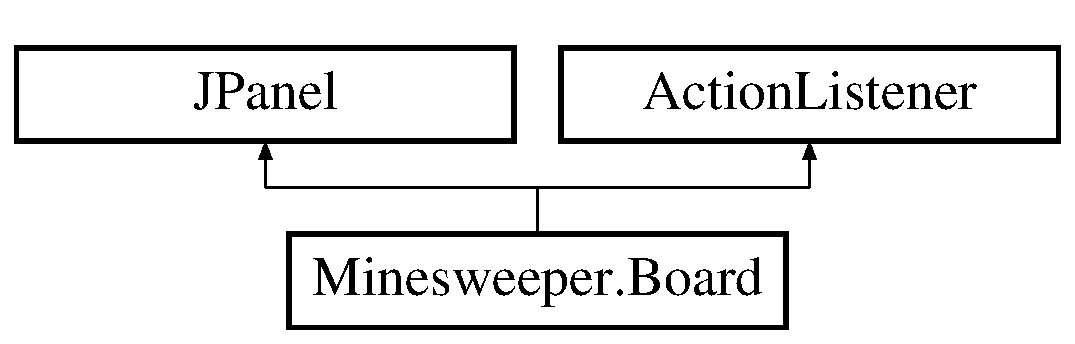
\includegraphics[height=2.000000cm]{class_minesweeper_1_1_board}
\end{center}
\end{figure}
\subsection*{Public Member Functions}
\begin{DoxyCompactItemize}
\item 
\mbox{\Hypertarget{class_minesweeper_1_1_board_a8a7b7d6303073fc6159a97bdf3ec9d91}\label{class_minesweeper_1_1_board_a8a7b7d6303073fc6159a97bdf3ec9d91}} 
void {\bfseries action\+Performed} (Action\+Event e)
\item 
\mbox{\Hypertarget{class_minesweeper_1_1_board_a44bb669c97a620f57b226561374984e1}\label{class_minesweeper_1_1_board_a44bb669c97a620f57b226561374984e1}} 
void {\bfseries show\+Neighbours} (\hyperlink{class_minesweeper_1_1_square}{Square} square)
\end{DoxyCompactItemize}


The documentation for this class was generated from the following file\+:\begin{DoxyCompactItemize}
\item 
Board.\+java\end{DoxyCompactItemize}

\hypertarget{class_minesweeper_1_1_main}{}\section{Minesweeper.\+Main Class Reference}
\label{class_minesweeper_1_1_main}\index{Minesweeper.\+Main@{Minesweeper.\+Main}}
Inheritance diagram for Minesweeper.\+Main\+:\begin{figure}[H]
\begin{center}
\leavevmode
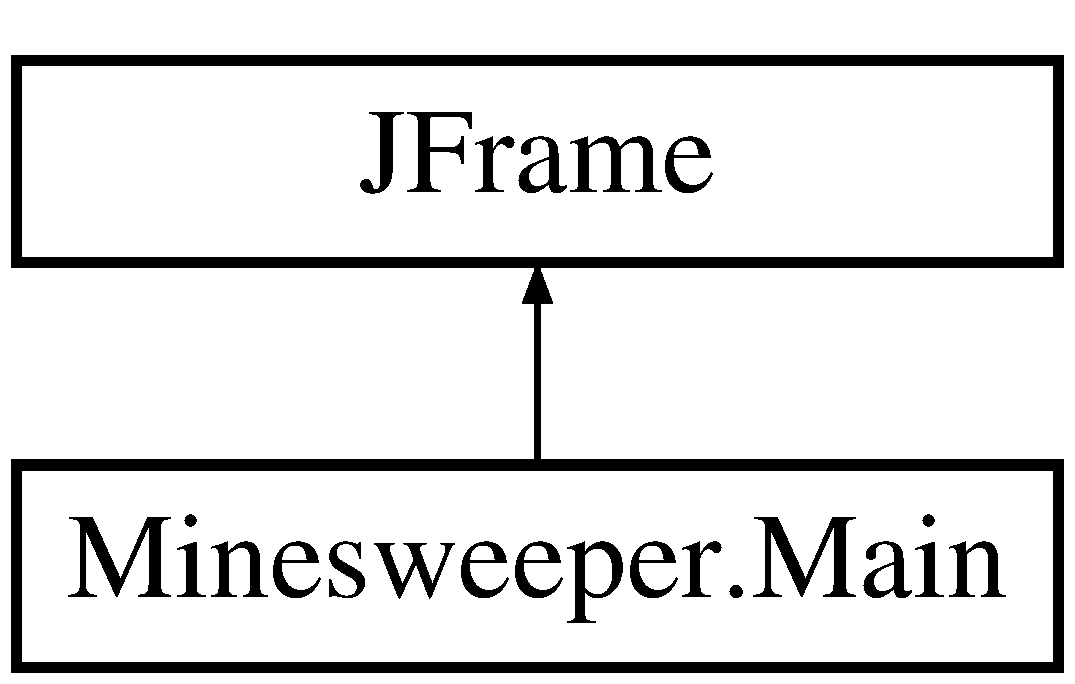
\includegraphics[height=2.000000cm]{class_minesweeper_1_1_main}
\end{center}
\end{figure}
\subsection*{Static Public Member Functions}
\begin{DoxyCompactItemize}
\item 
\mbox{\Hypertarget{class_minesweeper_1_1_main_adb90ffabc843f99f832232a3c0a7e192}\label{class_minesweeper_1_1_main_adb90ffabc843f99f832232a3c0a7e192}} 
static void {\bfseries main} (String\mbox{[}$\,$\mbox{]} args)
\end{DoxyCompactItemize}


The documentation for this class was generated from the following file\+:\begin{DoxyCompactItemize}
\item 
Main.\+java\end{DoxyCompactItemize}

\hypertarget{class_minesweeper_1_1_square}{}\section{Minesweeper.\+Square Class Reference}
\label{class_minesweeper_1_1_square}\index{Minesweeper.\+Square@{Minesweeper.\+Square}}
Inheritance diagram for Minesweeper.\+Square\+:\begin{figure}[H]
\begin{center}
\leavevmode
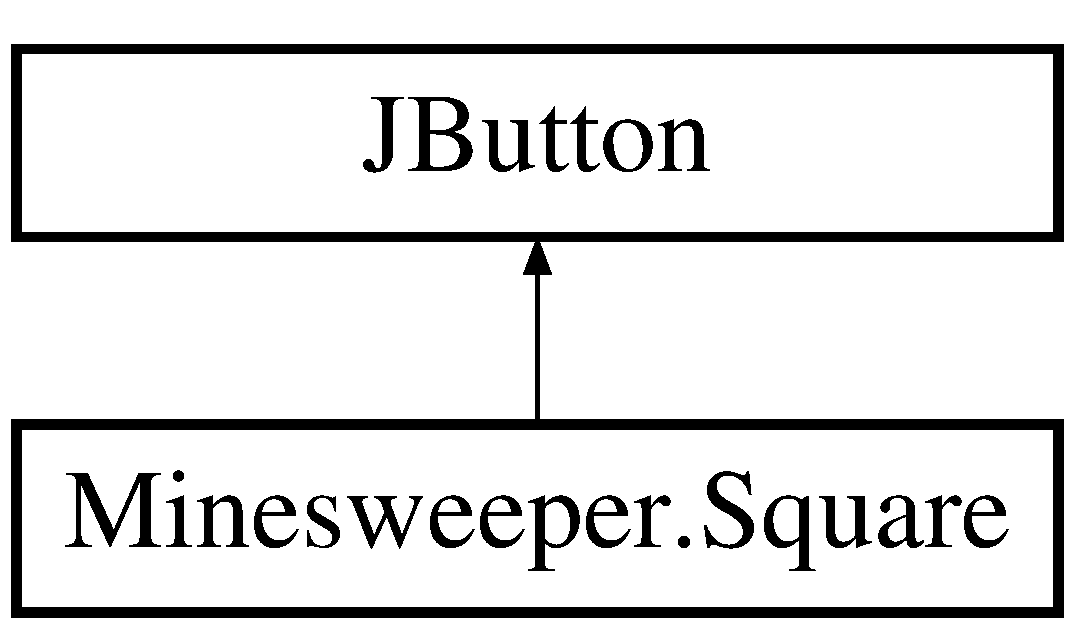
\includegraphics[height=2.000000cm]{class_minesweeper_1_1_square}
\end{center}
\end{figure}
\subsection*{Public Member Functions}
\begin{DoxyCompactItemize}
\item 
\mbox{\Hypertarget{class_minesweeper_1_1_square_a3e39a7f05b7c42865cf9844769352386}\label{class_minesweeper_1_1_square_a3e39a7f05b7c42865cf9844769352386}} 
{\bfseries Square} (int row, int col)
\item 
\mbox{\Hypertarget{class_minesweeper_1_1_square_a4bdd081dd7aa267ece7240dc3fcab06e}\label{class_minesweeper_1_1_square_a4bdd081dd7aa267ece7240dc3fcab06e}} 
void {\bfseries set\+Mine} ()
\item 
\mbox{\Hypertarget{class_minesweeper_1_1_square_ad0a380daf44435fbbb25b8067184664a}\label{class_minesweeper_1_1_square_ad0a380daf44435fbbb25b8067184664a}} 
boolean {\bfseries is\+Mine} ()
\item 
\mbox{\Hypertarget{class_minesweeper_1_1_square_ac89e00bfc6013521be4bcc0a5bb00b0b}\label{class_minesweeper_1_1_square_ac89e00bfc6013521be4bcc0a5bb00b0b}} 
boolean {\bfseries no\+Mines} ()
\item 
\mbox{\Hypertarget{class_minesweeper_1_1_square_a6fa68255c04a077ede4af229ec29c85a}\label{class_minesweeper_1_1_square_a6fa68255c04a077ede4af229ec29c85a}} 
void {\bfseries add\+Mine} ()
\item 
\mbox{\Hypertarget{class_minesweeper_1_1_square_aeaa596c8dd643bd7735fa13078947a3f}\label{class_minesweeper_1_1_square_aeaa596c8dd643bd7735fa13078947a3f}} 
int {\bfseries get\+Row} ()
\item 
\mbox{\Hypertarget{class_minesweeper_1_1_square_ac034763d2a72bd1161d57eaabd963ba6}\label{class_minesweeper_1_1_square_ac034763d2a72bd1161d57eaabd963ba6}} 
int {\bfseries get\+Column} ()
\item 
\mbox{\Hypertarget{class_minesweeper_1_1_square_a447093a2ff29144d18eeb99a8e452de3}\label{class_minesweeper_1_1_square_a447093a2ff29144d18eeb99a8e452de3}} 
int {\bfseries get\+Type} ()
\end{DoxyCompactItemize}


The documentation for this class was generated from the following file\+:\begin{DoxyCompactItemize}
\item 
Square.\+java\end{DoxyCompactItemize}

%--- End generated contents ---

% Index
\backmatter
\newpage
\phantomsection
\clearemptydoublepage
\addcontentsline{toc}{chapter}{Index}
\printindex

\end{document}
